% ----------------------------------------------------------------------- %
% Arquivo: cap2.tex
% ----------------------------------------------------------------------- %
\chapter{Fundamentação teórica}
\label{c_cap2}

\section{Introdução}
\label{s_c2_intro}

Este capítulo aborda os fundamentos teóricos sobre gestão de identidades. Os tópicos descritos nesse documento são: conceitos básicos de gestão de identidades, os modelos descritos na literatura, a especificação \ac{SAML}, e, por fim, será descrita a estrutura do \textit{framework} Shibboleth, principal componente de estudo deste trabalho.

\section{Gestão de Identidades}
\label{s_c2_gestaoid}

É perceptível a dificuldade de gerenciamento de identidades na rede de computadores, dificuldade proveniente da quantidade crescente de usuários e serviços disponibilizados. No entanto é importante situar num primeiro momento uma definição básica do que é identidade no mundo real, para então entender as dificuldades e necessidades para realização da gestão de identidades digitais.

De acordo com o Dicionário Aurélio, dentre os significados para palavra identidade, têm-se:
\textbf{Identidade} [\textit{Do Lat. escolástico identitate}]: \textit{S. f.} 2. Conjunto de caracteres próprios e exclusivo de uma pessoa, tais como nome, profissão, sexo, impressões digitais, defeitos físicos etc., o qual é considerado exclusivo dela e, consequentemente, considerado, quando ela precisa ser reconhecida. I. \textit{pessoal}: consciência que uma pessoa tem de si mesma \cite{ferreira:86}.

Segundo \cite{cao:10}, é difícil descrever o conceito de identidade uma vez que a definição de identidade está relacionada ao ambiente no qual esta é empregada, a contextos semânticos e a casos de uso. Como uma definição mais geral, tem-se que uma identidade é uma representação de uma entidade ou sujeito que seja suficiente para identificar esta entidade em um contexto particular \cite{maliki:07}. Uma entidade, por sua vez, é qualquer coisa existente no mundo real.

De acordo com a norma ITU-T Y.2720 \cite{itut:09}, uma identidade pode consistir de:

\begin{itemize}
 \item Identificador -- conjunto de caracteres e símbolos ou qualquer outra forma de dados usada para identificar unicamente uma identidade. Podem ser delimitados pelo tempo e/ou espaço. Por exemplo, uma \ac{URL} que é única ao longo do tempo. Também são exemplos de identificadores, o CPF, o  RG, o número de matrícula de uma instituição de ensino e o número do passaporte;
 \item Credenciais -- uma credencial é um atestado de qualificação, competência ou autoridade, que pode ser expedida por terceiros com autoridade relevante ou competência para tal ato e que atesta a veracidade da identidade. Na âmbito da computação, exemplo  de credenciais incluem certificados digitais X.509 assinados por uma autoridade certificadora, \ac{CA}, senha, asserções \ac{SAML}, entre outras;
 \item Atributos -- um conjunto de dados que descreve as características fundamentais de uma identidade. Como exemplo temos nome completo, endereço de domicílio, data de nascimento e papeis, (\textit{roles}).
\end{itemize}

A gestão de identidades pode ser entendida como o conjunto de processos e tecnologias usados para garantir a identidade de uma entidade ou de um objeto, garantir a qualidade das informações de uma identidade (identificadores, credenciais e atributos) e para prover procedimentos de autenticacão, autorização, contabilização e auditoria \cite{itut:09}. A gestão de identidades também envolve aspectos relacionados com a definição, certificação e gerenciamento do ciclo de vida das identidades digitais, infraestruturas para troca e validação dessas informaçãoes, juntamente com os aspectos legais \cite{pope:05, chadwick:09}.

No final da década de 90, a infraestrutura de gestão de identidades se destinava à provisão de serviços, especialmente serviços centralizados de autenticação. Neste cenário, as organizações (empresas ou universidades) empregavam serviços de diretórios baseados em \ac{LDAP}. Esses serviços eram destinados a fornecer mecanismos de autenticação de forma centralizada, com o objetivo de facilitar a gerência deste ambiente e prover uma forma de autenticação única, conhecida como \acf{SSO} \cite{suess:09}.

Para a realização da gestão de identidades é necessária a construção de um sistema integrado de políticas e processos, infraestrutura para validação e troca de credenciais entre os envolvidos, além das definições, certificação e gerenciamento do ciclo de vida das identidades digitais que permita o tratamento e manipulação de identidades (atributos de identidades) \cite{josan:05, chadwick:09}.

Segundo \apud{damiani:03}{wangham:10b} uma lista de requisitos, com o intuito de garantir uma melhor experiência para os usuários, deve ser contemplada considerando que a facilidade provida para o usuário não afete a segurança das informações pessoais. A seguir, tem-se os requisitos listados por \cite{damiani:03}:
\begin{itemize}
 \item Interoperabilidade -- As identidades dos usuários devem ser representadas em um formato comum, possibilitando que estas possam ser compreendidas e validadas em diferentes domínios administrativos e de segurança;
 \item Mecanismo para revogação de identidades -- O sistema deverá prover uma forma para que os usuários possam gerencias as informações contidas em suas identidades, assim como revogá-las quando desejado;
 \item Gerenciamento de confiança -- Relações de confiança entre provedores de serviços e de identidades de diferentes domínios permitem que identidades emitidas em um sejam aceitas em outro. Para esse tipo de interação, é preciso prover uma forma de indicar o nível de confiança associado a cada relação, sendo que este influenciará no comportamento dos provedores de serviço;
 \item Privacidade -- Os usuários devem possuir meios de expressar suas preferências de privacidade sobre as informações pessoais presentes em suas identidades, e quais serão disponibilizada na relação entre os diferentes provedores;
 \item Anonimato -- Aos usuários deve ser garantido o direito de permanecerem anônimos de forma que as informações fornecidades com sua identidade digital não possam ser usadas para obter dados de suas outras identidades. Para garantir o anonimato, pode-se utilizar pseudônimos.
\end{itemize}

Em \apud{bhargav:07}{wangham:10b}, um sistema de gerenciamento de identidades é caracterizado pelos seguintes elementos:

\begin{itemize}
 \item Usuário -- quem deseja acessar algum serviço.
 \item Identidade -- conjunto de atributos de um usuário. Por exemplo, nome, filiação, data de nascimento, endereço, etc. Complementando, uma asserção de atributos consiste em uma declaração, emitida por um terceiro confiável, indicando que uma determinada entidade possui os referidos atributos \cite{wangham:10b};
 \item Provedor de identidades (IdP) -- responsável por emitir a identidade de um usuário. Após o usuário passar por um processo de autenticação, este recebe um token, que é reconhecido como válido pelos provedores de serviço;
 \item Provedor de serviço (SP) -- oferece recursos a usuários autorizados, após verificar o token de autenticação e após comprovar que a mesma carrega todos os atributos necessários para o acesso.
\end{itemize}

\subsection{Modelos de gestão de identidade}
\label{ss_c2_modelos}

Os modelos de gestão de identidade são classificados de acordo com a sua arquitetura. Em \cite{josan:05, pope:05, bhargav:07}, classificam os modelos de gestão de identidades como tradicional, federado, centralizado e centrado no usuário. Cada um desses modelos apresenta uma forma diferente de interação.

A Figura \ref{fig_1} ilustra os modelos de gestão de identidades e uma breve descrição destes modelos é apresentada a seguir:

\begin{itemize}
 \item Tradicional (ou isolado) -- a identificação do usuário é tratada de forma isolada por cada provedor de serviços, o qual também atua como provedor de identidades (ver Figura \ref{fig_1}.a). Cabe ao usuário criar uma identidade digital para cada provedor de serviço que deseja interagir, não havendo assim o compartilhamento das identidades desses usuários entre diferentes provedores de serviços;
 \item Federado -- os provedores de identidades e provedores serviços, podem estar em domínios diferentes, permitindo que usuários que possuam suas credenciais em um provedor de identidade acesse um serviço disponível num provedor de serviço em outro domínio (ver Figura \ref{fig_1}.b). Este modelo permite que os usuários possuam uma única identidade e não precisem lidar com o processo de autenticação diversas vezes, graças ao conceito de autenticação única (SSO);
 \item Centralizado -- só existe um único provedor de identidades o qual é responsável por autenticar os usuários, fornecer aos provedores de serviços informações sobre estes e todos os provedores de serviços devem confiar plenamente nas informações fornecidas por este provedor de identidades (ver Figura \ref{fig_1}.c); 
 \item Centrado no usuário -- tem por objetivo dar ao usuário o controle sobre suas identidades digitais. Na proposta de \cite{pope:05} as identidades de um usuário, destinadas a diferentes provedores de serviços, são armazenadas em um dispositivo físico que fica em poder do usuário, como um \textit{smartcard} ou mesmo um telefone celular (ver Figura \ref{fig_1}.d).
\end{itemize}

\begin{figure}[!ht]
 \centering
 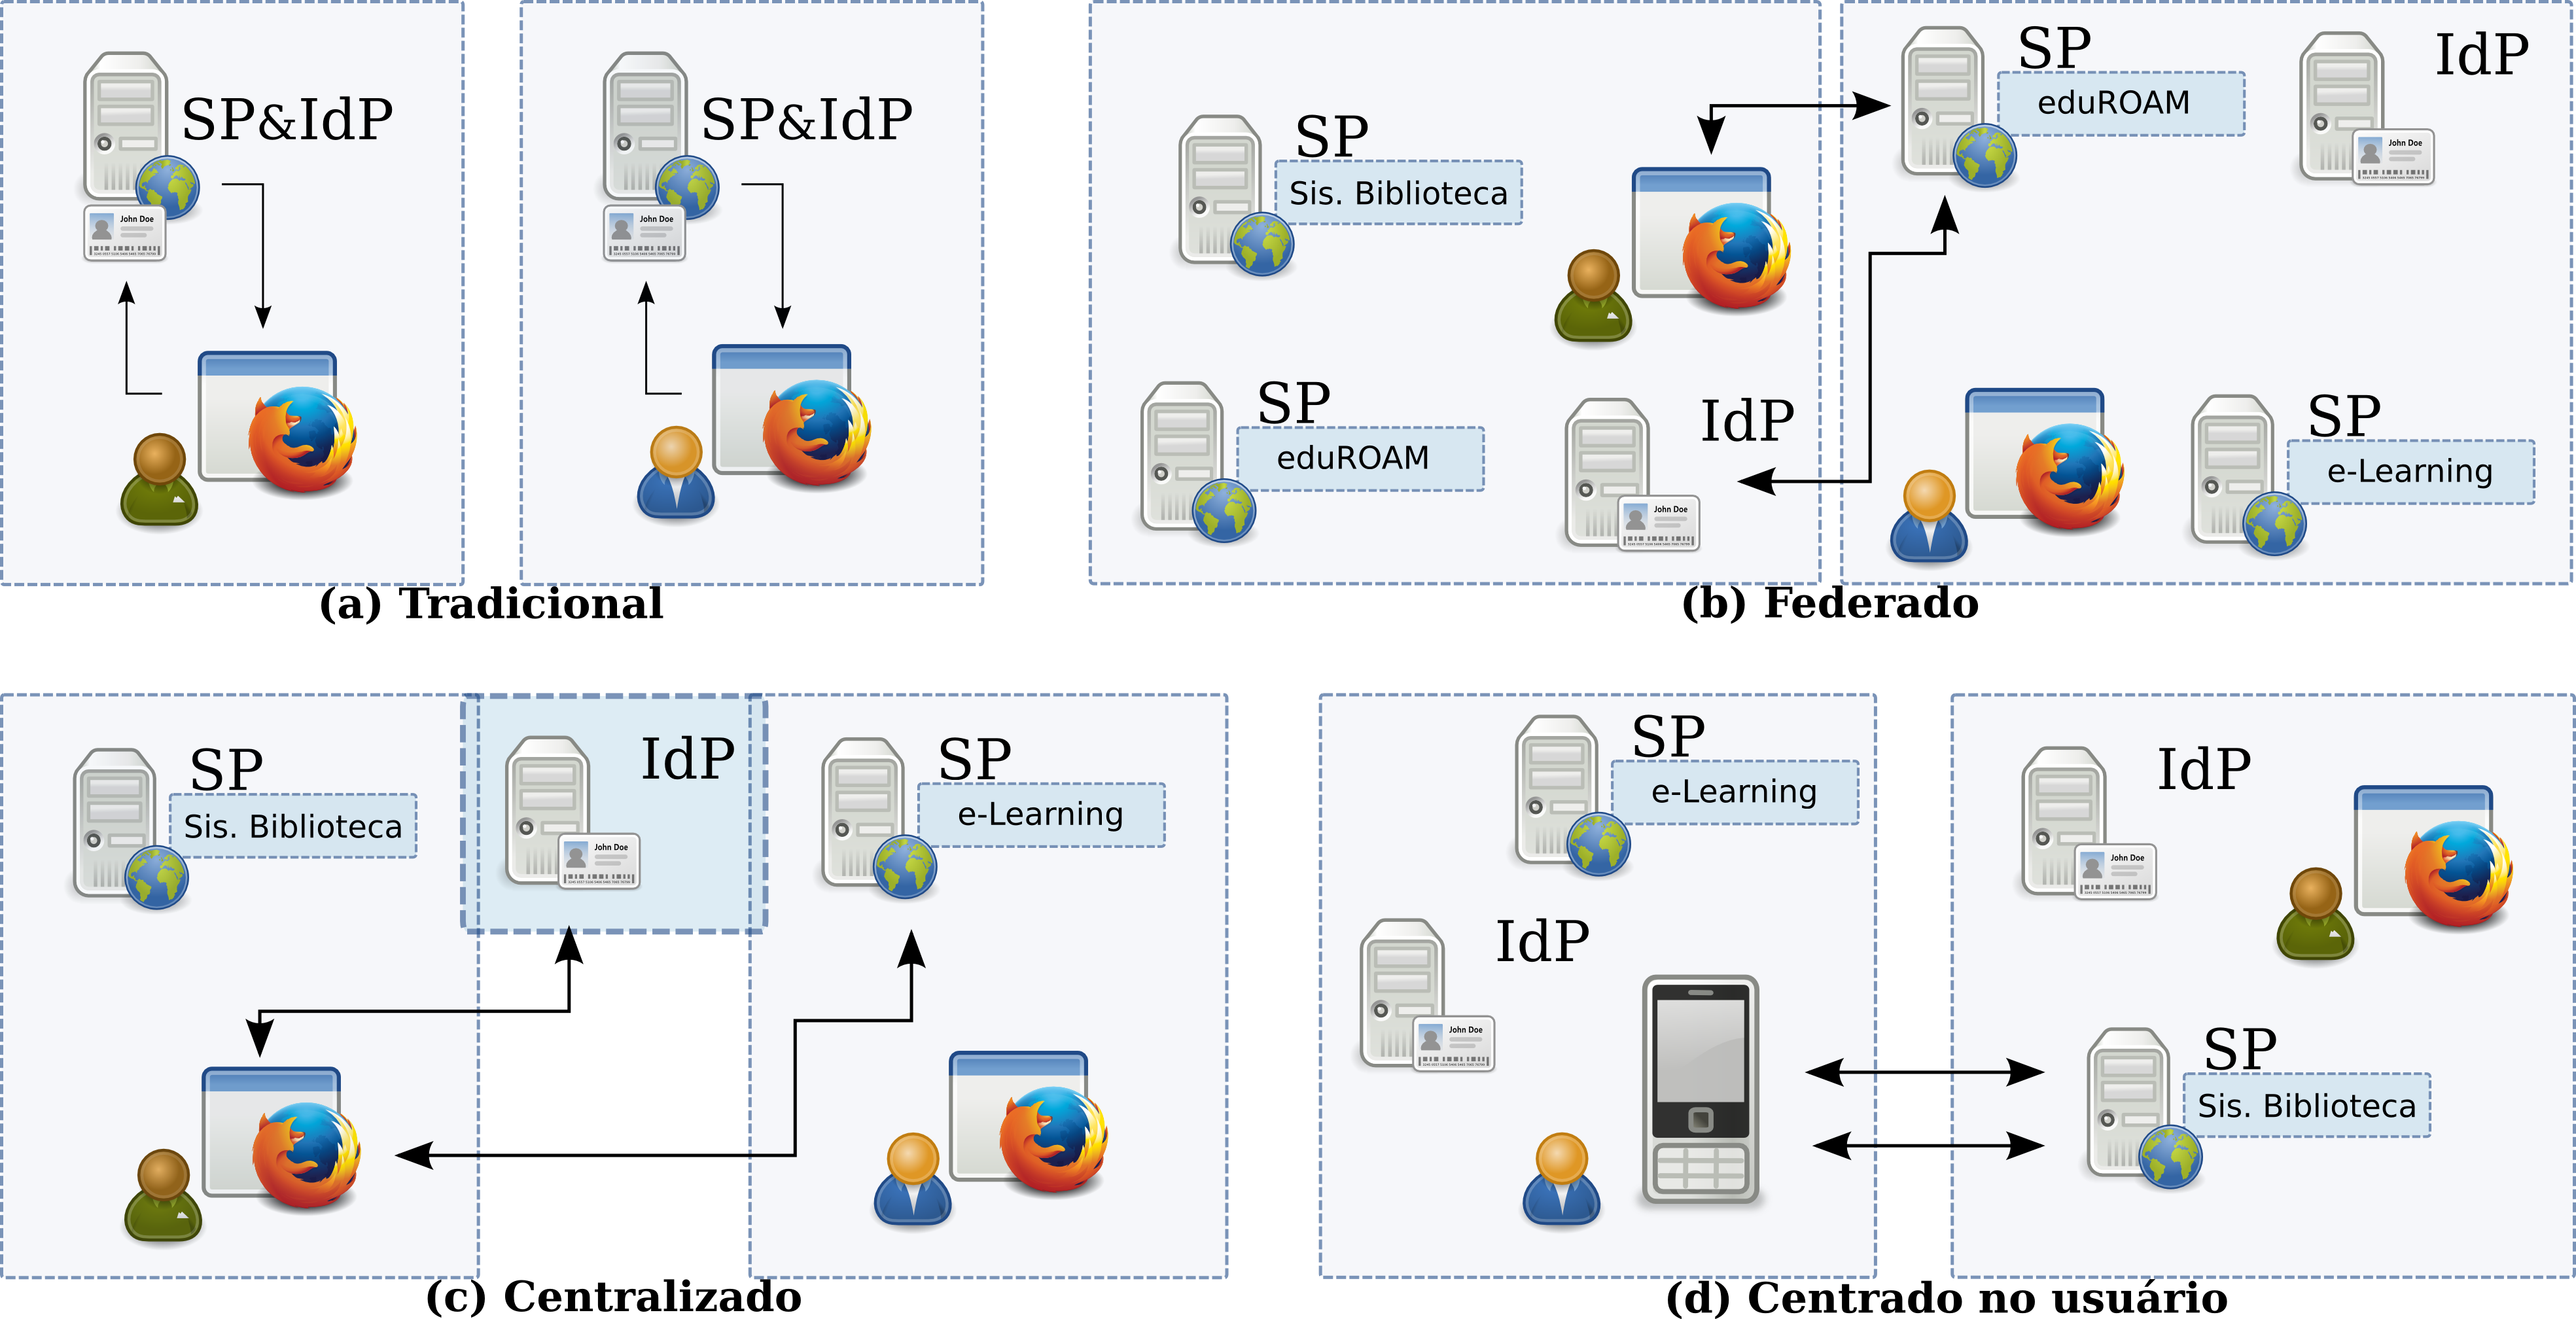
\includegraphics[width=1\textwidth]{figuras/modelos-gid.png}
 \caption{Modelos de Gestão de Identidade.}
 \label{fig_1}
\end{figure}

Dentre os modelos apresentados, é possível realizar algumas considerações quanto as suas características, por exemplo o modelo tradicional é amplamente utilizado nos atuais sistemas computacionais presentes na Internet. No entanto, apesar de ser amplamente utilizado seu uso tende a ser custoso tanto para o usuário quanto para os provedores de serviços. Implicando que os usuários possuam múltiplas identidades para interagir entre os diferentes serviços, como o servidor de e-mails, \textit{site} de notícias, livrarias, e outros. Cada provedor de serviços pode exigir um conjunto próprio de atributos para compor a identidade digital do usuário. Por outro lado, um conjunto comum de atributos pode ser exigido por diversos provedores de serviços, como nome da conta, senha, endereço, data de nascimento, etc. \cite{mello:09}.

O modelo centralizado trata destes problemas apontados sobre o modelo tradicional. O modelo centralizado fundamentalmente tem o compartilhamento de identidades dos usuários entre os provedores de serviços e no conceito de autenticação única (SSO), porém todas as identidades estão centralizadas num único  provedor de identidade, que detém o poder de todas as identidades, e podendo gerar discordâncias entre confiabilidade do uso destas pelo IdP \cite{wangham:10b}.

O modelo de gestão identidades federadas é uma abordagem que visa otimizar a troca de informações relacionadas a identidade por meio de relações de confiança construídas nas federações \cite{camenisch:07}. Os acordos estabelecidos entre provedores de identidades e de serviços garantem que identidades emitidas em um domínio sejam reconhecidas por provedores de serviços de outros domínios e o conceito de autenticação única é garantido mesmo diante de diferentes domínios \cite{wangham:10b}.

As principais propostas e implementações do modelo centrado no usuário fazem uso de um dos modelos apresentados anteriormente, sendo o modelo de identidade federadas o mais usado. O usuário se autentica neste dispositivo físico e cabe a este liberar as informações do usuário para cada provedor de serviços que o usuário acessar, respeitando totalmente as preferências de privacidade do usuário \cite{wangham:10b}.

\section{Especificações SAML}
\label{s_c2_saml}

A \acf{SAML} é uma especificação que define uma infraestrutura para troca de informações seguras da autenticação do usuário, seus direitos e atributos entre parceiros (instituições) na rede de computadores. A especificação SAML é elaborada pelo \ac{SSTC} que faz parte da \ac{OASIS}. A especificação SAML apresenta informações de segurança na forma de asserções (declarações). A especificação SAML define as regras e a sintaxe para geração, requisição, transferências e uso dessas asserções \cite{wangham:10b, oasis:08}.

As mensagens SAML são codificadas em arquivos XML que geralmente são incorporados em outras estruturas para o transporte, como por exemplo, o HTTP POST ou mensagens \ac{SOAP} codificadas. Esse tipo de transporte é denominado na especificação como \textit{binding}. A especificação SAML fornece um conjunto base de perfis para o uso de afirmações e protocolos, visando possibilitar a interoperabilidade no uso dos recursos SAML \cite{oasis:08, macaneiro:13}.

Atualmente, a especificação SAML está na versão 2.0 (lançada em 2005) e é o padrão mais adotado que concretiza o modelo de identidades federadas. Os sistemas de gerenciamento de identidades que utilizam a especificação SAML, o fazem por funcionalidades que estão disponíveis no padrão. A especificação SAML é utilizada de diferentes maneiras, as mais relevantes estão descritas em \cite{oasis:08}, tais como:

\begin{itemize}
 \item Web SSO -- a SAML possibilita o SSO por meio da comunicação de uma asserção de autenticação em um primeiro local para um segundo local que confia na origem da autenticação;
 \item Autorização baseada em atributos -- a especificação SAML permite a autorização baseada em atributos para comunicar informações de uma identidade entre diferentes \textit{web sites}, possibilitando desta forma apoio em algumas transações;
 \item Segurança em Serviços Web -- as asserções SAML podem ser usadas dentro das mensagens SOAP, afim de realizar operações com segurança de informações e identidade entre agentes em um serviço \textit{web}.
\end{itemize}

A especificação SAML é composta por alguns componentes que funcionam como blocos que podem ser combinados em configurações diferentes para suportar implementações de cenários diferentes. Os componentes primeiramente permitem transferência de identidade, autenticação, atributos e informações de autorização entre provedores de identidades e de serviços que possuem uma relação de confiança estabelecida. O núcleo da especificação SAML define a estrutura e o conteúdo das asserções e mensagens de protocolo usado para transferir essas informações \cite{oasis:08}.

\subsection{Componentes SAML}
\label{ss_c2_comp_saml}

Segundo \cite{oasis:08}, a especificação SAML é composta por componentes responsáveis por informações específicas, protocolos utilizados para troca dessas informações assim como os tipos de ligações que podem ser realizadas para o estabelecimento da comunicação entre elementos de uma federação.

A SAML define três tipos diferentes de declarações de afirmações que podem ser criadas por uma autoridade SAML. A estrutura e o conteúdo de uma asserção são definidos por meio de um esquema XML.

A asserção (\textit{assertion}) é usualmente criada por uma parte declarante (\textit{asserting party}) baseada em uma requisição da parte confiante (\textit{relying party}). No entanto, sob certas circunstâncias a asserção pode ser encaminhada para um parte confiante mesmo se não foi solicitada. Uma asserção é um pacote de informação que fornece uma ou mais declarações feitas por uma autoridade SAML. Uma asserção é composta basicamente por um conjunto de informações que são, a entidade da asserção, as condições usadas para validar a asserção e as declarações sobre o sujeito. Uma asserção pode conter três tipos de declarações:

\begin{itemize}
 \item Autenticação -- são geradas pela entidade que autentica o usuário. Possuem pelo menos o método de autenticação e de data e hora da autenticação;
 \item Decisão de autorização -- que especifica as permissões que o usuário tem no sistema, e que pode ser autorizada ou negada;
 \item Atributos -- que contêm informações específicas do usuário.
\end{itemize}

Os protocolos (\textit{protocols}) são mensagens de solicitações e respostas que os provedores de serviços podem utilizar. Os protocolos descritos na especificação SAML são:

\begin{itemize}
 \item protocolo de pedidos de autenticação;
 \item protocolo de consulta e pedido de asserção;
 \item protocolo para encerramento de sessão;
 \item protocolo para resolução de artefatos;
 \item protocolo de gerenciamento de identificador de nome;
 \item protocolo de mapeamento de identificador de nome.
\end{itemize}

As ligações (\textit{bindings}) SAML, são utilizadas pelos protocolos para transporte de mensagens entre as partes do sistema usando padrões de comunicação já estabelecidos. Na versão 2.0 da SAML estão disponíveis diversas ligações, dentre estas as mais comuns são:

\begin{itemize}
 \item HTTP \textit{Redirect Binding} -- o \textit{binding} HTTP \textit{Redirect} fornece um meio para transmitir asserções SAML dentro da URL de uma solicitação HTTP. Esta opção pode ser utilizada quando não é possível um caminho direto entre um provedor de identidade e um provedor de serviços. Neste caso a mensagem SAML será transportada de maneira indireta, normalmente, via o navegador web do usuário final;
 \item HTTP POST \textit{Binding} -- nesse modelo de \textit{binding}, as mensagens SAML são transmitidas dentro do conteúdo de um formulário HTML, utilizando do método HTTP POST para postar o SAML em um provedor de serviços;
 \item HTTP \textit{Artifact Binding} -- este modelo de \textit{binding} denominado de “Artefato HTTP SAML” fornece um mecanismo que permite a comunicação por intermédio de um agente do usuário HTTP intermediário. Esta ligação tem o objetivo de reduzir o fluxo de mensagens por meio do SAML;
 \item URI \textit{Binding} -- este modelo de \textit{binding} possibilita que uma asserção SAML específica seja repassada ao provedor de serviço por intermédio de uma HTTP URI;
 \item SOAP \textit{Binding} -- o SOAP é um protocolo de comunicação baseado no formato XML. É um protocolo simples, extensível e flexível, desenvolvido como um padrão W3C, importante no desenvolvimento de aplicações para permitir comunicação entre programas pela internet.
\end{itemize}

Os perfis (\textit{profiles}) SAML possibilitam que os protocolos do SAML e suas asserções trabalhem em fluxos de dados específicos, por exemplo, com a finalidade de promover a funcionalidade de gerenciamento de identidades e autenticação única (SSO). Existem também perfis de atributos (\textit{Attribute Profiles}) que não se referem a nenhuma mensagem de protocolo ou ligação, que definem como realizar a transmissão de informações de atributos usando asserções, de forma que se enquandre em usos comuns para diferentes tipos de ambientes (ex. X500, LDAP, DCE).

Na figura \ref{fig_2} é possível visualizar a pilha de componentes SAML conforme descritas anteriormente.

\begin{figure}[!ht]
 \centering
 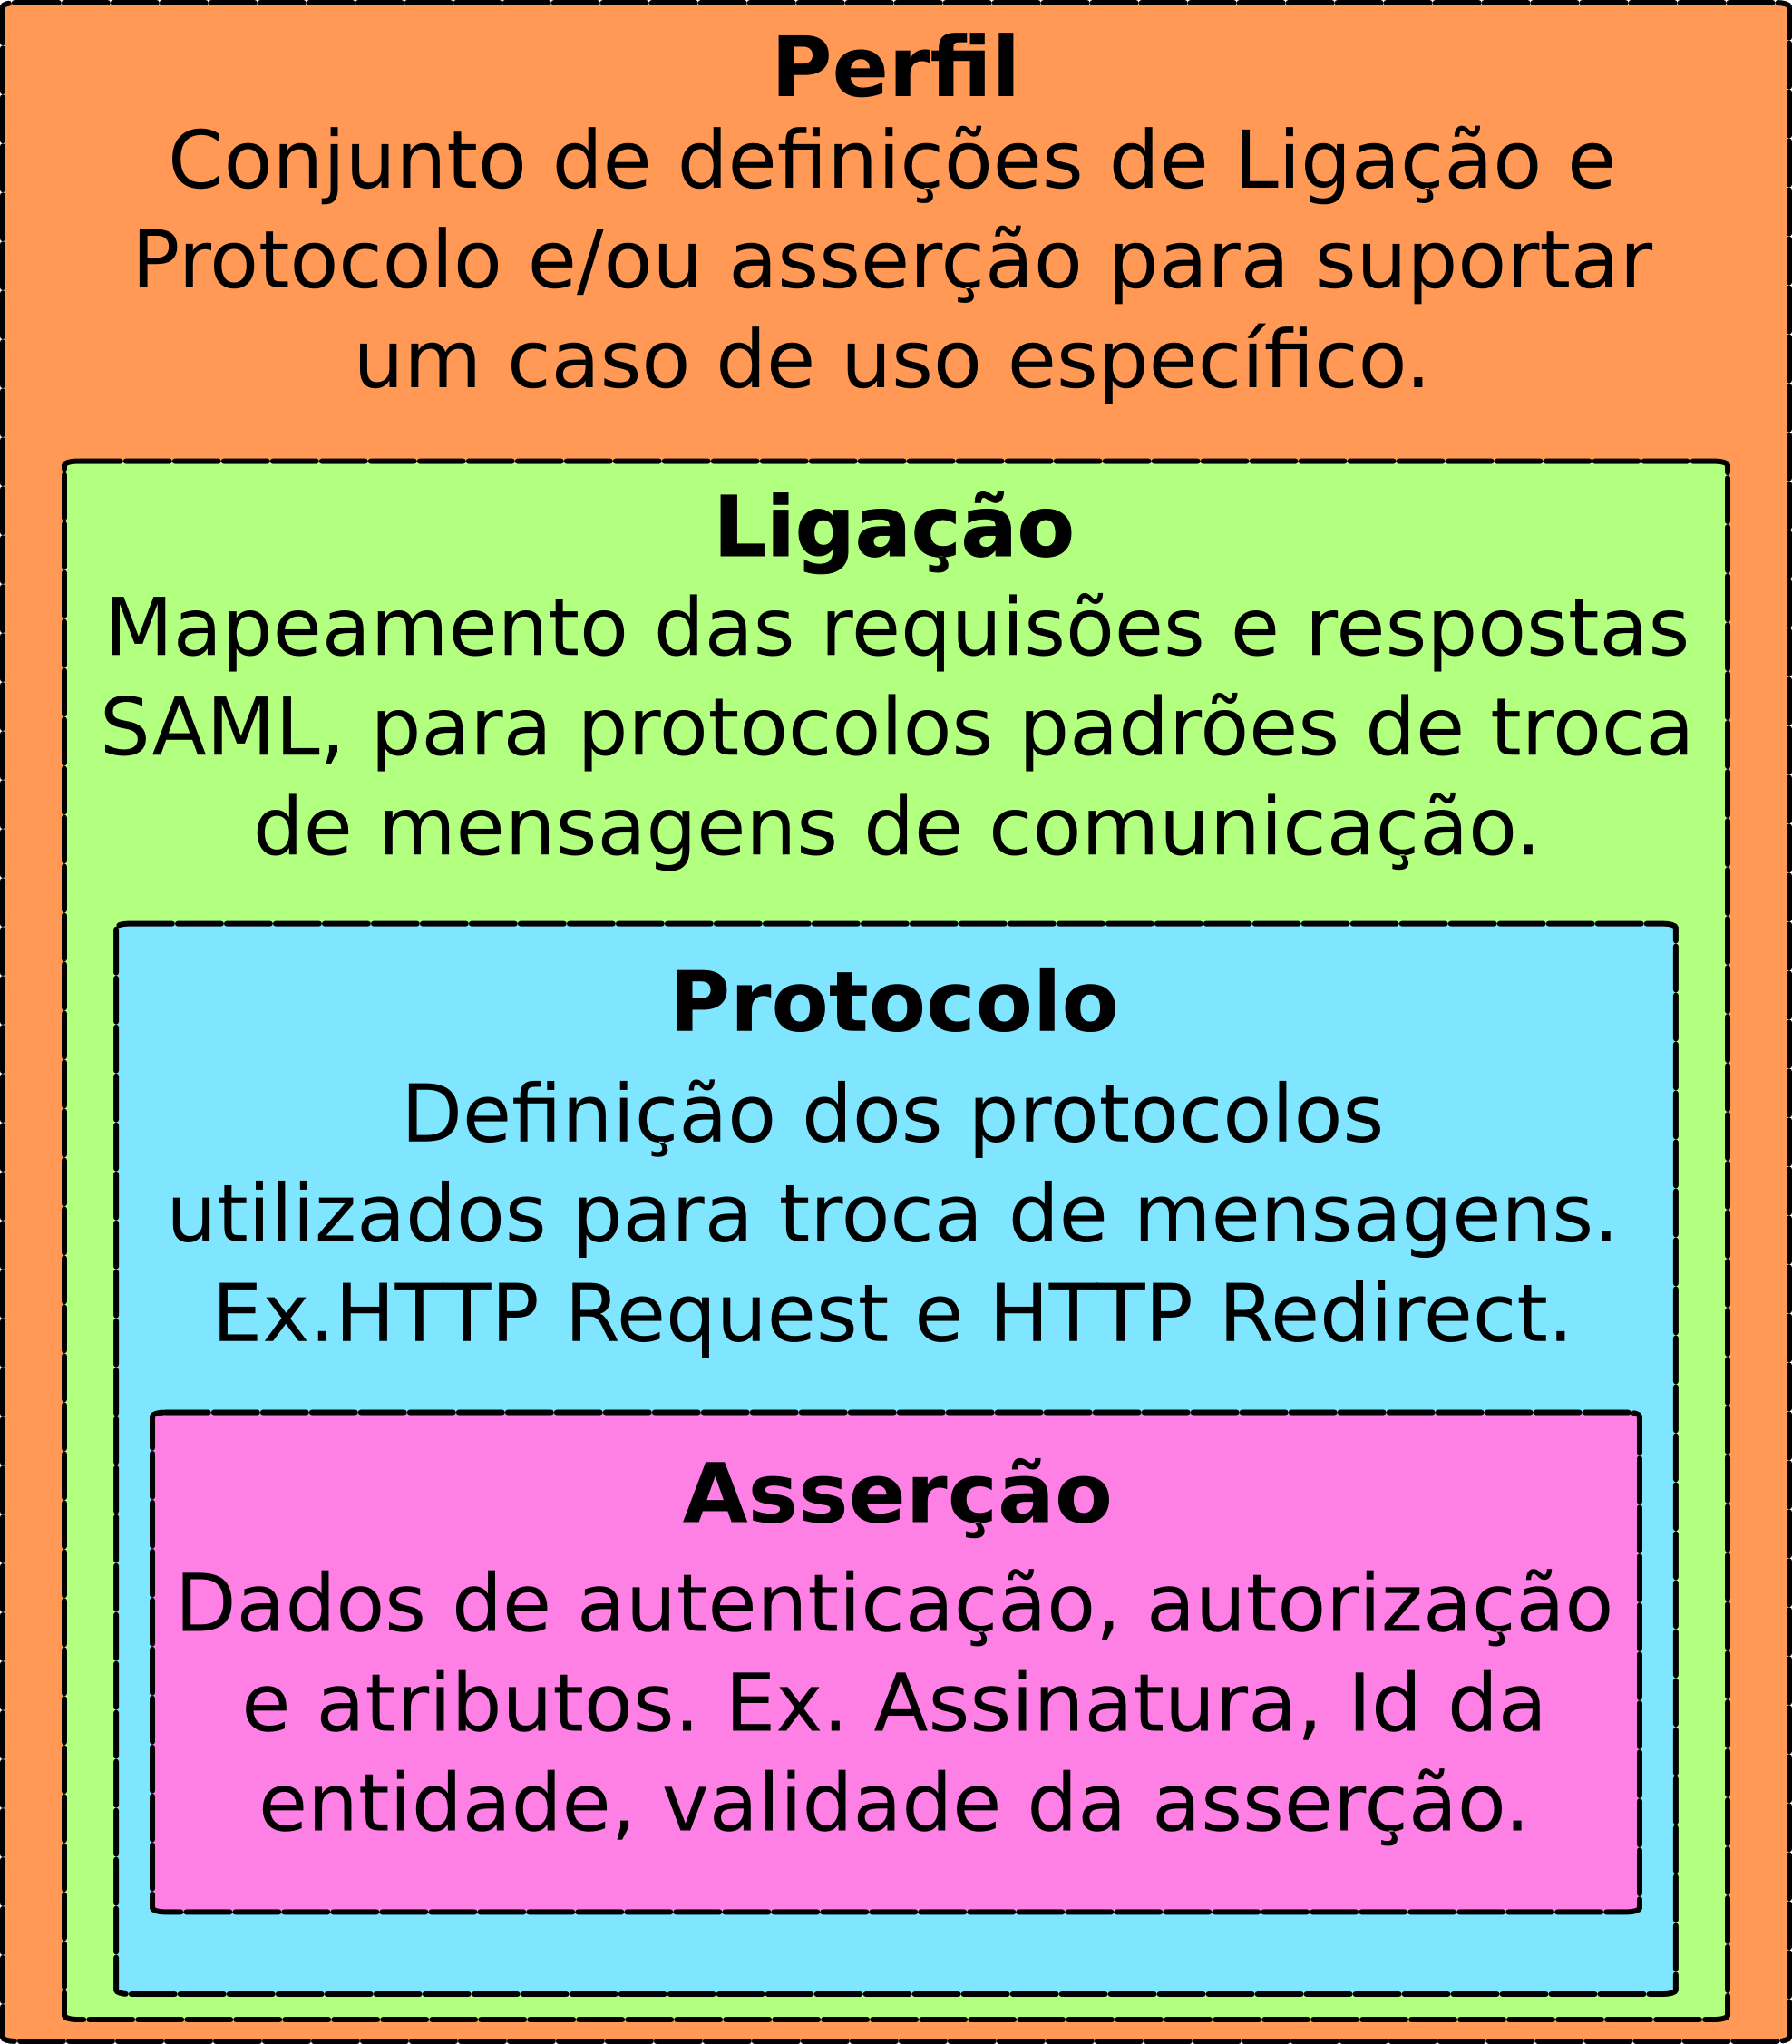
\includegraphics[width=0.6\textwidth]{figuras/pilha-saml.png}
 \caption{Pilha de componentes SAML.}
 \label{fig_2}
\end{figure}

Dois outros componentes bastante utilizados para composição de ambientes SAML, são:

\begin{itemize}
 \item Metadado -- que define como informar e compartilhar informações entre entidades SAML e papéis (como IdP, SP, etc.). O metadado contém informações sobre ligações SAML, identificadores de identidade, protocolos de transportes suportados, certificados digitais e chaves criptográficas; e
 \item Contexto de Autenticação -- em inúmeras ocasiões um provedor de serviço pode necessitar de informações detalhadas referente ao mecanismo de autenticação que é empregado pelo provedor de identidade do usuário. O contexto de autenticação SAML é usado para comunicação entre o provedor de serviços e o de identidades, permitindo ao primeiro solicitar uma forma específica de autenticação e ao segundo permitir o acesso do usuário em seus serviços \cite{oasis:08}.
\end{itemize}

\section{Framework Shibboleth}
\label{s_c2_framework}

O termo ``shibboleth'' denota uma palavra usada para distinguir pessoas de grupos distintos. A origem do termo remete ao velho testamento (Juízes, 12:1-15), onde ele foi usado para distinguir duas tribos semitas, os gileaditas e os efremitas, que travaram uma grande batalha. O gileaditas, vencedores, bloquearam a passagem do Jordão para evitar que os efremitas sobreviventes pudessem escapar. As sentinelas exigiam que todos o passante dissesse ``shibboleth''; como os efremitas não tinham o fonema \/x\/ em seu dialeto, só conseguiam pronunciar ``siboleth'' (com \/si\/ na primeira sílaba), eram identificas e executados \cite{moreira:11}.

O projeto \textit{Shibboleth} \cite{scavo:05} foi uma iniciativa do consórcio americano Internet2\footnote{http://www.internet2.edu/} que teve como principal objetivo lançar uma implementação de código aberto, baseada em padrões abertos, para tratar desafios relacionados ao gerenciamento de identidades e controle de acesso em instituições acadêmicas \cite{wangham:10a}.

O projeto \textit{Shibboleth} teve inicio em 2000 no comitê \ac{MACE}. O projeto do \textit{framework} se prolongou por um ano.  O \textit{framework} Shibboleth 1.0  foi lançado em Julho de 2003, em Agosto de 2005 foi lançado a versão 1.3, e por último (até ao momento) foi lançado a versão 2.0 em Março de 2008 \cite{manuel:09}. Já existem \textit{cases} oficiais de desenvolvimento de uma nova versão\footnote{http://shibboleth.net/documents/business-case.pdf}, com melhorias e novas implementações.

Com o amadurecimento do \textit{framework} Shibboleth, constata-se que este provê um sistema de gerenciamento de identidades federadas possível de ser adotado não só no âmbito acadêmico, mas também no governamental, e privado (comércio eletrônico).

Uma federação \textit{Shibboleth} é composta por um grupo de organizações e tem como princípio um conjunto de práticas comuns e de mecanismos de segurança e permissões previamentes definidas o que permite a participação \cite{carmody:05}.

O framework está fundamentado sobre padrões abertos como o XML e a SAML e provê uma forma fácil para que aplicações \textit{web} usufruam das facilidades providas pelo modelo de identidades federadas, como o conceito de autenticação única (SSO) e a troca segura de atributos dos usuários por todos provedores de serviços que compõem a federação \cite{wangham:10b}.

\subsection{Esquema brEduPerson}
\label{ss_c2_breduperson}

O \textit{framework} Shibboleth provê suporte a uma classe de atributos (\textit{Object Class}) chamado \textit{eduPerson}, que é um esquema LDAP, originalmente desenvolvida por \cite{internet2:08} baseado nas RFCs 2256\footnote{https://www.ietf.org/rfc/rfc2256.txt} e 2798\footnote{https://www.ietf.org/rfc/rfc2798.txt} \cite{wahl:97, smith:00}, respectivamente. É um conjunto padrão de atributos de identidades comuns para federações acadêmicas. Esta classe define quais atributos, informações, do usuário são necessárias para um funcionamento harmonioso entre IdP e SP dentro do escopo de uma instituição acadêmica. 

Usando como base este conjunto de atributos \textit{eduPerson} a RNP propôs uma adaptação deste esquema para as universidades e instituições brasileiras, e o denominou \textit{brEduPerson}. A gestão do esquema brEduPerson se dá conforme a figura \ref{fig_3}.

\begin{figure}[!htpb]
 \centering
 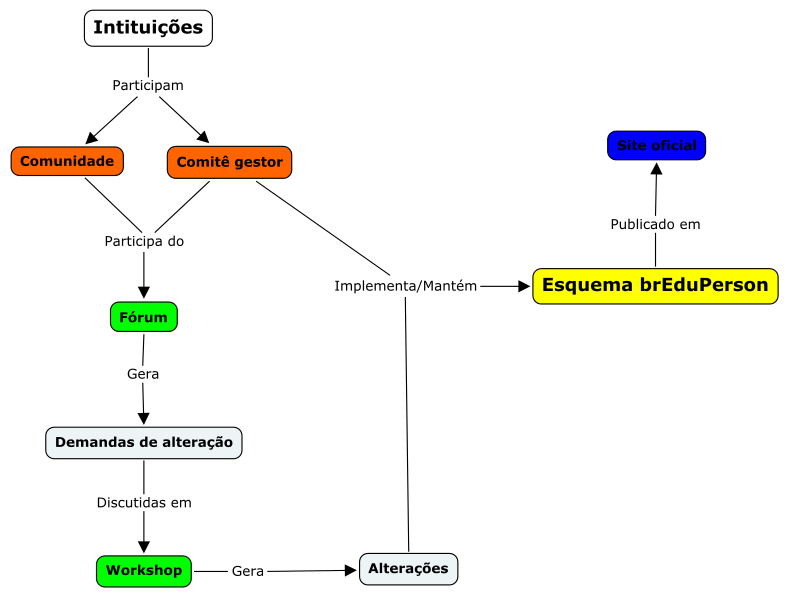
\includegraphics[width=0.8\textwidth]{figuras/gestao-breduperson.png}
 \caption{Gestão do esquema brEduPerson. Fonte: Esquema brEduPerson.}
 \label{fig_3}
\end{figure}

O esquema \textit{brEduPerson} visa complementar o conjunto original de esquemas que descrevem informações sobre pessoas, o \textit{inetOrgPerson}, o \textit{eduPerson} e o esquema \ac{SCHAC} definido por \cite{terena:09}. Este esquema armazena informações específicas para a realidade do país, tais como informações genéricas de qualquer cidadão residente no Brasil, (como CPF, Endereço, Passaporte), informações gerais sobre os membros de uma instituição (e-mail, cargo entre outros) além de informações específicas sobre os funcionários e alunos destas instituições. Tendo estas características definidas a RNP define que 6 atributos são altamente recomendados, 10 são sugeridos e 25 são opcionais\footnote{http://wiki.rnp.br/download/attachments/41190038/BrEduPersonv1
0.pdf}.

\subsubsection{Estrutura do esquema brEduPerson}
\label{ss_c2_estrut_breduperson}

Para o uso de um esquema em instituições de ensino e pesquisa, é necessário modelar relacionamentos entre conjuntos de informações. É preciso poder capturar na estrutura de diretórios LDAP o fato de uma mesma pessoa poder desempenhar diferentes papéis, como de um aluno (que também pode estar desempenhando uma pesquisa), e a cada um dos quais está associada uma data de ingresso, um código de curso, uma matrícula, e outras informações, ou que uma mesma pessoa pode ter direito a vários números \acs{VoIP}, cada um deles com suas características \cite{rnp:09}. Para modelar esses relacionamentos, a RNP optou por usar uma solução hierárquica.

Os nós em um diretório LDAP formam uma árvore. Cada nó, independentemente de originar algum outro nó na árvore, é uma entrada com suas próprias informações (atributos). Esses nós são por vezes chamados de \textit{containers} na terminologia X.500.

O item principal (uma pessoa) tem uma ligação com uma instituição de ensino e/ou pesquisa com o qual se deseja relacionar as demais informações deste vínculo, este item será tratado como um \textit{container} e abaixo deste aparecerão nós com as informações relacionadas. As informações genéricas (nome, cpf, e-mail, tipo de vínculo, etc), aparecerão como entradas, sobre ela, pois cada pessoa pode ter diferentes vínculos com a instituição, como vínculo de estudante em curso, vínculo de funcionário, etc. Ainda, abaixo da entrada com dados gerais podem aparecer diversas entradas descrevendo telefones VoIP, dados biométricos, formas de contato, como e-mail, telefone pessoal etc \cite{rnp:09}.

\subsubsection{eduPerson e brEduPerson}
A classe de objetos \textit{eduPerson} foi criada no contexto do Projeto Internet2\footnote{https://www.internet2.edu} para descrever indivíduos da comunidade acadêmica. O nome \textit{brEduPerson} é utilizado para descrever a classe de objetos que representa um vínculo com a instituição por ser o objeto cujos campos mais se assemelham aos da classe \textit{eduPerson}. O \textit{eduPerson}, no entanto, supõe apenas uma entrada por pessoa, com campos multivalorados descrevendo, por exemplo, os diversos vínculos de um indivíduo com a instituição. Esse modelo não satisfez as necessidades da Federação CAFe, pois era necessário associar a cada vínculo existente (professor, estudante, funcionário, etc) outras informações, como a data de entrada e saída. No esquema \textit{brEduPerson}, tanto a entrada principal de cada indivíduo (de classe estrutural \textit{brPerson}) como cada entrada abaixo dessa que descreve um vínculo (de classe estrutural \textit{brEduPerson}) têm a classe \textit{eduPerson} como auxiliar, 
pois atributos gerais do indivíduo ficam na entrada principal enquanto que os atributos relativos a um de seus vínculos ficam na entrada específica de vínculo \cite{rnp:09}. Na figura \ref{fig_4} é possível visualizar a distribuição dos atributos de uma pessoa, e seus vínculos.

\begin{figure}[!htpb]
 \centering
 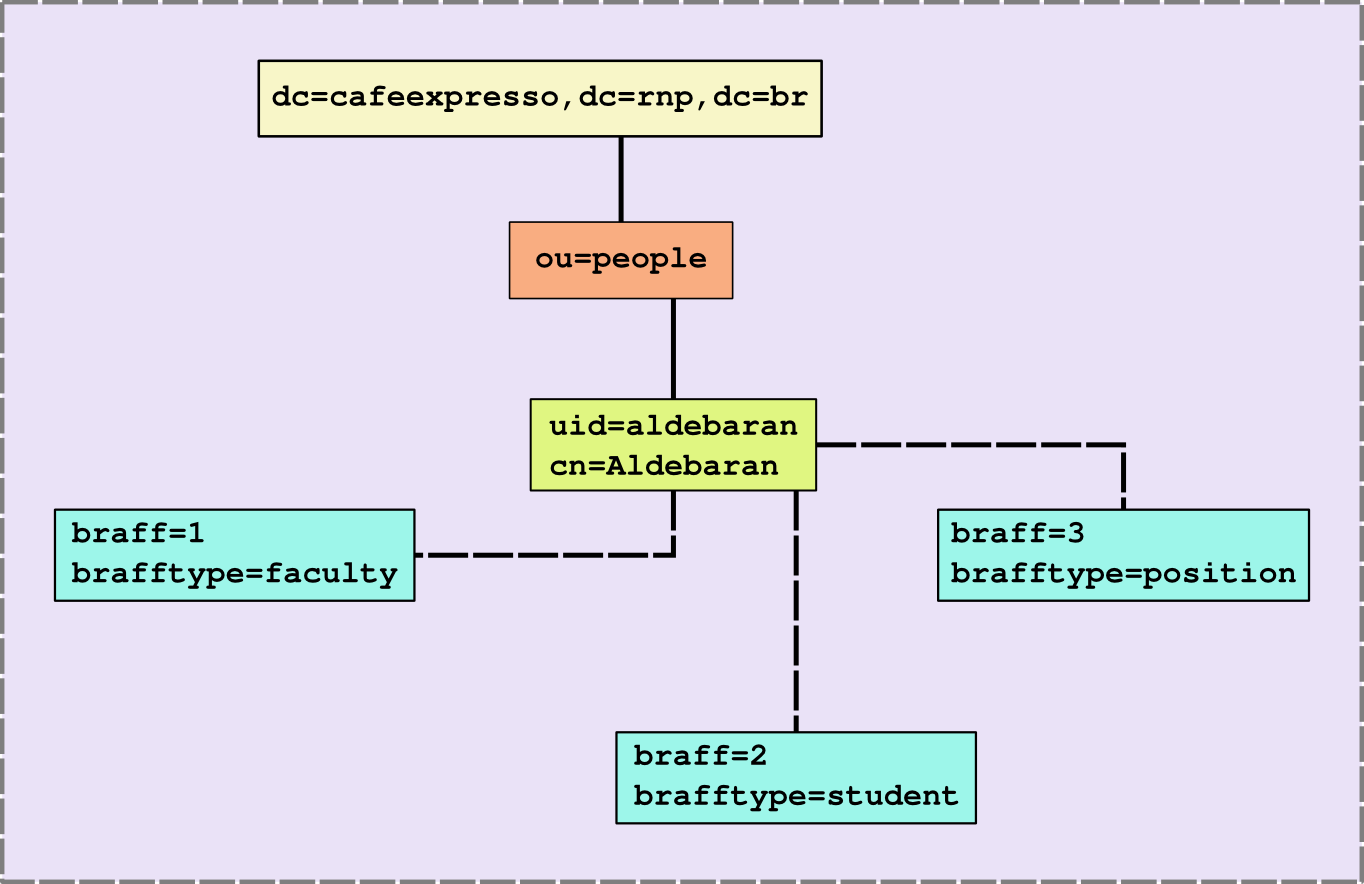
\includegraphics[width=0.8\textwidth]{figuras/arvore-breduperson.png}
 \caption{Árvore de atributos do brEduPerson.}
 \label{fig_4}
\end{figure}

Em um ambiente federado, a padronização destes atributos é fundamental para que provedores de serviços saibam quais atributos poderão requisitar e para que provedores de identidades saibam quais atributos deverão fornecer \cite{wangham:10a}.

\subsection{Provedores Shibboleth}
\label{s_c2_provedores}

O \textit{framework} Shibboleth é composto por dois provedores, que são chamados provedor de identidades, \acf{IdP}, e provedor de serviços, \acf{SP}. Estes são os principais compontes do framework. O IdP é a entidade responsável pelo gerenciamento das identidades dos usuários, seus atributos, gerenciamento da autenticação e declarações de atributos. Enquanto o SP é a entidade responsável pelo gerenciamento de segurança dos serviços disponibilizados, que, com base nas declarações de atributos recebidas do IdP, permite o acesso a estes serviços. A autorização para acesso ao serviço requisitado ainda passa por um conceito utilizado pelo \textit{framework} Shibboleth, dito contexto de segurança, que precisa ser estabelecido para um usuário, por meio da relação de confiança estabelecida entre SP e IdP, que permitirá o acesso seguro ao serviço \cite{kallela:08}.

No \textit{framework} Shibboleth, o processo de autenticação é executado na instituição de origem do usuário, por meio de seu provedor de identidades, fazendo uso dos mecanismos de autenticação presentes nesta instituição. A autenticação de usuários pode ser feita por meio de senhas, de tickets Kerberos, certificados X.509, entre outros mecanismos \cite{chadwick:09, wangham:10b}.

Um IdP é dividido em quatro subcomponentes \cite{scavo:05}:

\begin{itemize}
 \item Autoridade de autenticação -- serviço definido por meio da especificação SAML responsável por emitir pedidos de autenticação requisitado pela parte confiante (\textit{relying parties}), neste caso, o SP;
 \item Serviço de autenticação única (SSO) -- processo para a manipulação de requisições de autenticação de um usuário. Este componente obtém as requisições de asserção e gera um fomulário HTML que é redicionado para o SP;
 \item Serviço de resolução de artefatos -- um artefato é uma referência para uma asserção de autenticação. O SP define um perfil que utiliza a troca de asserções por referência, a resolução de artefatos (\textit{artifact binding}) é responsável por tratar estas requisições. O IdP ao invés de enviar a asserção de resposta de autenticação via navegador do usuário, envia uma asserção de referência a asserção expedida;
 \item Autoridade de atributos -- componente responsável pela emissão de asserções de atributos baseadas nas requisições dos provedores de serviços. Antes da edição de qualquer asserção, a autenticação e autorização das requisições recebidas precisam ser realidas.
\end{itemize}

Um SP assim como o IdP é formado por subcomponentes, são estes \cite{scavo:05}:

\begin{itemize}
 \item Recurso alvo --  os recursos Web são protegidos no SP por meio de serviços de Controle de Acesso, o que impede usuários não autenticados/autorizados de acessarem esses recursos;
 \item Serviço consumidor de asserção -- gerencia as funções de SSO no provedor de serviço. Processa a asserção de atributos recebida ou o artefato, podendo elaborar requisições de asserções de atributos adicionais, estabele contexto de segurança e redirecionada o usuário para o serviço em ambiente seguro;
 \item Requisitante de atributos -- realiza interações com a autoridade de atributos do IdP, para realizar trocas adicionais de atributos, uma vez que um contexto de segurança tenha sido estabelecido. Esse tipo de interação ocorre diretamente entre os provedores, por meio dos protocolos de ligação (\textit{binding}) SAML, e não utilizam o navegador Web do cliente.
\end{itemize}

Adicionalmente, um terceiro componente é especificado no \textit{framework} Shibboleth, o serviço de descoberta ou \acf{DS}. Na CAFe Expresso foi implantado dois tipos diferentes de DS, o \acf{WAYF} e o \acf{EDS}. Ambos os serviços, WAYF e EDS realizam o redirecionamento do usuário entre o provedor de serviços e o provedor de identidades. Uma vez que o provedor de serviço não sabe, nem tem obrigação de saber, qual o provedor de identidades que o usuário utiliza para validar seus credenciais de autenticação. O WAYF mantém uma base dos provedores utilizando metadados SAML, que além de realizar o estabelecimento de relação de confiança entre os provedores, provê o redirecionamento do usuário para seu provedor de identidade de origem \cite{shibb:05, kallela:08, wangham:10b}. O EDS no entanto permite o uso da mesma base disponibilizada pelo WAYF, porém o processo de redirecionamento do usuário entre SP, EDS e IdP é transparente para o usuário. Além do que, o EDS é embutido diretamente na página do SP, diminuindo 
ainda mais os redirecionamentos entre páginas \textit{web}.

\begin{figure}[!htpb]
 \centering
 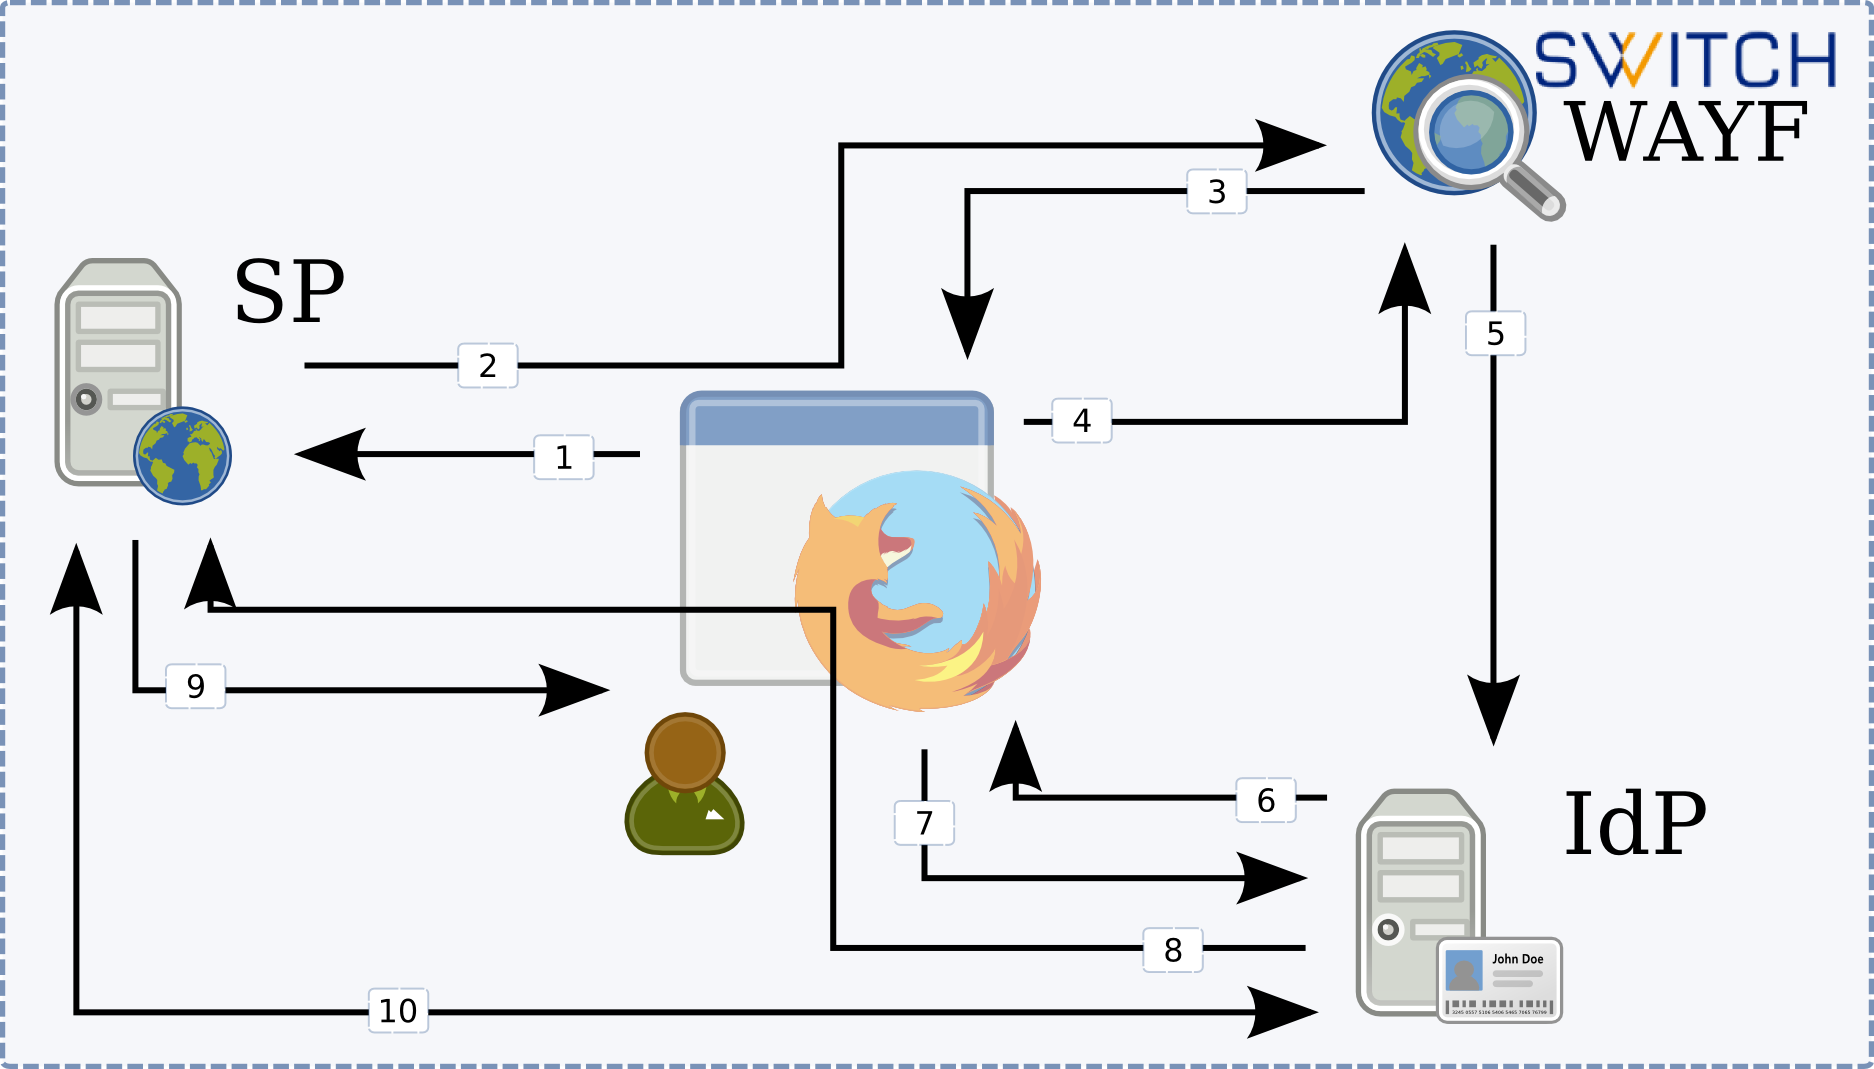
\includegraphics[width=0.8\textwidth]{figuras/fluxo-shibboleth.png}
 \caption{Fluxo de mensagens entre usuários e provedores Shibboleth.}
 \label{fig_5}
\end{figure}

A Figura \ref{fig_5} exemplifica o fluxo de mensagens trocadas entre os provedores quando um usuário realiza a requisição de um serviço a um provedor de serviços da federação, conforme descritos a seguir \cite{feliciano:11}:

\begin{itemize}
 \item Passo 1 -- O usuário através do navegador web solicita acesso a um serviço protegido por um provedor de serviços da federação;
 \item Passo 2, o provedor de serviços recebe a requisição e redireciona o navegador do usuário  para o serviço de descoberta ou DS;
 \item Passo 3, o DS apresenta uma lista de IdPs da federação;
 \item Passo 4, o usuário informa o seu provedor de identidades;
 \item Passo 5, o DS atualiza o cookie de sessão com as informações do IdP escolhido e redireciona o navegador do usuário para o IdP indicado;
 \item Passo 6, o serviço de SSO é requisitado no IdP escolhido e este adquire uma declaração de autenticação (asserção SAML) da Autoridade de Autenticação, que retorna a asserção SAML gerada para o navegador do usuário;
 \item Passo 7, o usuário fornece as suas credenciais por meio de uma mensagem HTTP POST para o IdP de origem;
 \item Passo 8, o IdP autentica o usuário e uma asserção SAML é retornada para o navegador do usuário e o serviço consumidor de asserção do SP processa a resposta da autenticação. O contexto de segurança é criado no SP e redirecionamento do usuário para o recurso solicitado;
 \item Passo 9, opcionalmente, o provedor de serviço pode enviar um pedido de atributos ao provedor de identidade do usuário;
 \item Por fim, no passo 10, o provedor de identidade retorna os valores dos atributos requisitados.
\end{itemize}